% !Mode:: "TeX:UTF-8"
% !TEX program  = xelatex

\section{实验结果与分析}
\label{sec:results}

\subsection{主结果}

下文按问题类型汇总主结果，分别报告 TSP 与 CVRP
在合成混合数据集和 LIB 基准数据集上的表现。

\subsubsection{TSP 结果}

\begin{table}[htb]
  \centering
  \caption{TSP 上的结果：合成混合数据集与 TSPLIB}
  \label{tab:tsp-main-results}
  \small
  \begin{tabular}{@{}p{4.5cm}cccc@{}}
    \toprule
    & \multicolumn{2}{c}{合成混合数据集（1000 实例）} & \multicolumn{2}{c}{TSPLIB（49 实例）} \\
    \cmidrule(lr){2-3}\cmidrule(lr){4-5}
    方法 & mean length $\downarrow$ & top-1 accuracy $\uparrow$ & mean length $\downarrow$ & top-1 accuracy $\uparrow$ \\
    \midrule
    \textbf{Oracle} & 7.8699 & 1.0000 & 8.1422 & 1.0000 \\
    \textbf{Neural-LinUCB} & \textbf{7.9420} & 0.2930 & \textbf{8.2116} & \textbf{0.4490} \\
    \textbf{SingleBest} & 7.9578 & 0.1720 & 8.2334 & 0.1020 \\
    t2t500 & 7.9578 & 0.1720 & 8.2334 & 0.1020 \\
    difusco500 & 7.9580 & 0.1180 & 8.2473 & 0.0612 \\
    t2t & 7.9646 & 0.1110 & 8.2404 & 0.1224 \\
    difusco & 7.9939 & 0.0490 & 8.2645 & 0.0408 \\
    bq & 7.9953 & \textbf{0.3000} & 8.2731 & \textbf{0.4490} \\
    lehd & 8.0365 & 0.1720 & 8.2599 & 0.0816 \\
    elg & 8.0894 & 0.0780 & 8.3842 & 0.1429 \\
    \bottomrule
  \end{tabular}
\end{table}

表 \ref{tab:tsp-main-results} 汇总了 TSP 在合成混合数据集和 TSPLIB 上的结果。
在合成混合数据集上，Neural-LinUCB 取得了最低的非 Oracle mean length，
优于 SingleBest 基线；
但在 top-1 accuracy 上，\texttt{bq} 略高于 Neural-LinUCB，
说明当前基于排名的 reward 学到的选择策略与最终 mean length 最优并不完全一致。
在 TSPLIB 上，Neural-LinUCB 仍然取得最低的非 Oracle mean length，
并与 \texttt{bq} 在 top-1 accuracy 上并列最高，
表明该方法在 TSP 上具备一定的分布外泛化能力。

\subsubsection{CVRP 结果}

\begin{table}[htb]
  \centering
  \caption{CVRP 上的结果：合成混合数据集与 CVRPLIB}
  \label{tab:cvrp-main-results}
  \small
  \begin{tabular}{@{}p{4.5cm}cccc@{}}
    \toprule
    & \multicolumn{2}{c}{合成混合数据集（1000 实例）} & \multicolumn{2}{c}{CVRPLIB（100 实例）} \\
    \cmidrule(lr){2-3}\cmidrule(lr){4-5}
    方法 & mean length $\downarrow$ & top-1 accuracy $\uparrow$ & mean length $\downarrow$ & top-1 accuracy $\uparrow$ \\
    \midrule
    \textbf{Oracle} & 18.1781 & 1.0000 & 68.3098 & 1.0000 \\
    \textbf{Neural-LinUCB} & \textbf{18.2785} & \textbf{0.5770} & 73.7296 & 0.3800 \\
    \textbf{SingleBest} & 18.4167 & 0.4170 & \textbf{68.7926} & \textbf{0.4200} \\
    omni & 18.4167 & 0.4170 & 69.0533 & 0.3100 \\
    bq & 18.6225 & 0.2050 & 72.4496 & 0.1500 \\
    lehd & 18.6556 & 0.2520 & 77.2945 & 0.1100 \\
    elg & 18.6643 & 0.0770 & \textbf{68.7926} & \textbf{0.4200} \\
    mvmoe & 19.6954 & 0.0490 & 76.1748 & 0.0100 \\
    \bottomrule
  \end{tabular}
\end{table}

表 \ref{tab:cvrp-main-results} 汇总了 CVRP 在合成混合数据集和 CVRPLIB 上的结果。
在合成混合数据集上，Neural-LinUCB 在 mean length 和 top-1 accuracy 上都优于固定单方法，
说明实例条件化选择在同分布设定下是有效的。
相比之下，在 CVRPLIB 上，Neural-LinUCB 的 mean length 为 73.7296，
高于 \texttt{elg}， \texttt{omni} 与 \texttt{bq}。
这说明当前方法在 CVRP 上泛化能力不足。

\subsection{训练损失曲线}

图 \ref{fig:training-loss} 给出了 Neural-LinUCB 在合成混合数据集训练过程中的平均 loss 变化。
loss 在训练过程中持续下降，说明当前训练流程在数值上是稳定的；
但在 step 6000 之后基本进入平台期，loss 不再下降。
这一现象与前文关于排名 reward 局限性的分析是一致的，即排名 reward 不能很好的区分不同实例。

\begin{figure}[htb]
  \centering
  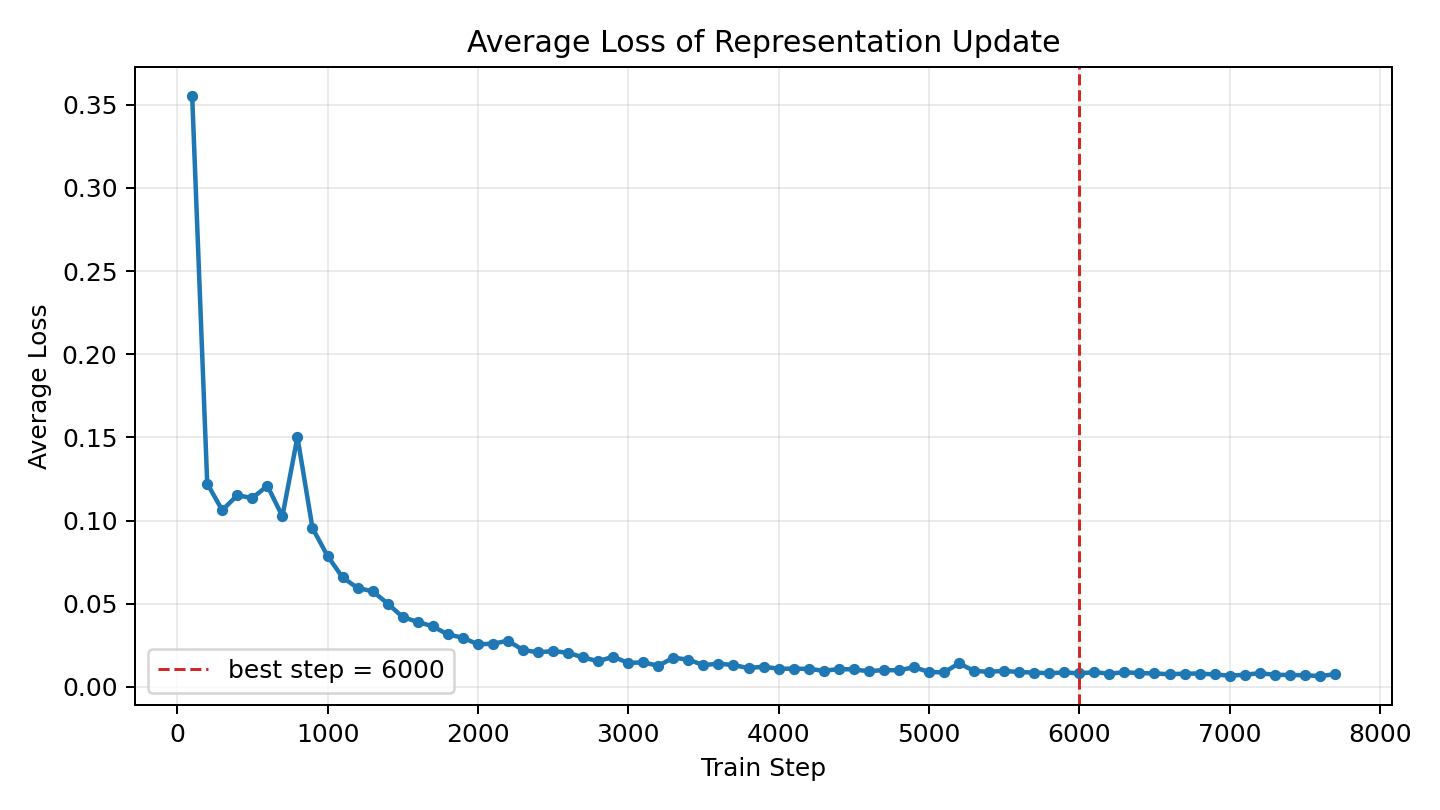
\includegraphics[width=0.82\textwidth]{figures/research/figure-06-training-loss.png}
  \caption{Neural-LinUCB 在合成混合数据集训练过程中的 loss 曲线}
  \label{fig:training-loss}
\end{figure}

\subsection{负结果分析}

在确定初始化选择框架之前，本文尝试过多种决策粒度设定，
表 \ref{tab:research-evolution} 列出了其中三条具有代表性的路径。

\begin{table}[htb]
  \centering
  \caption{不同决策建模路径的比较}
  \label{tab:research-evolution}
  \small
  \begin{tabular}{ll}
    \toprule
    研究路径 & 决策粒度 \\
    \midrule
    双门控强化学习 & 初始化一次 + 迭代器一次 \\
    步级算子选择 & 初始化一次 + 每步选算子 \\
    初始化选择 & 初始化一次 \\
    \bottomrule
  \end{tabular}
\end{table}

前两类设定都出现了策略坍缩，以双门控强化学习为例。

\paragraph{双门控强化学习的快速坍缩}
图 \ref{fig:two-gate-collapse} 显示，在双门控强化学习原型中，初始化选择最终固定到 \texttt{elg}，
迭代阶段则在中途迅速切换并固定到 \texttt{rrc\_lehd\_10}，评测 mean length 只在这一切换附近出现一次跃迁，随后基本不再变化。
这说明双门控方案在当前动作设计和奖励条件下很容易退化为少数固定组合。步级算子选择中也观察到了类似现象。

\begin{figure}[htb]
  \centering
  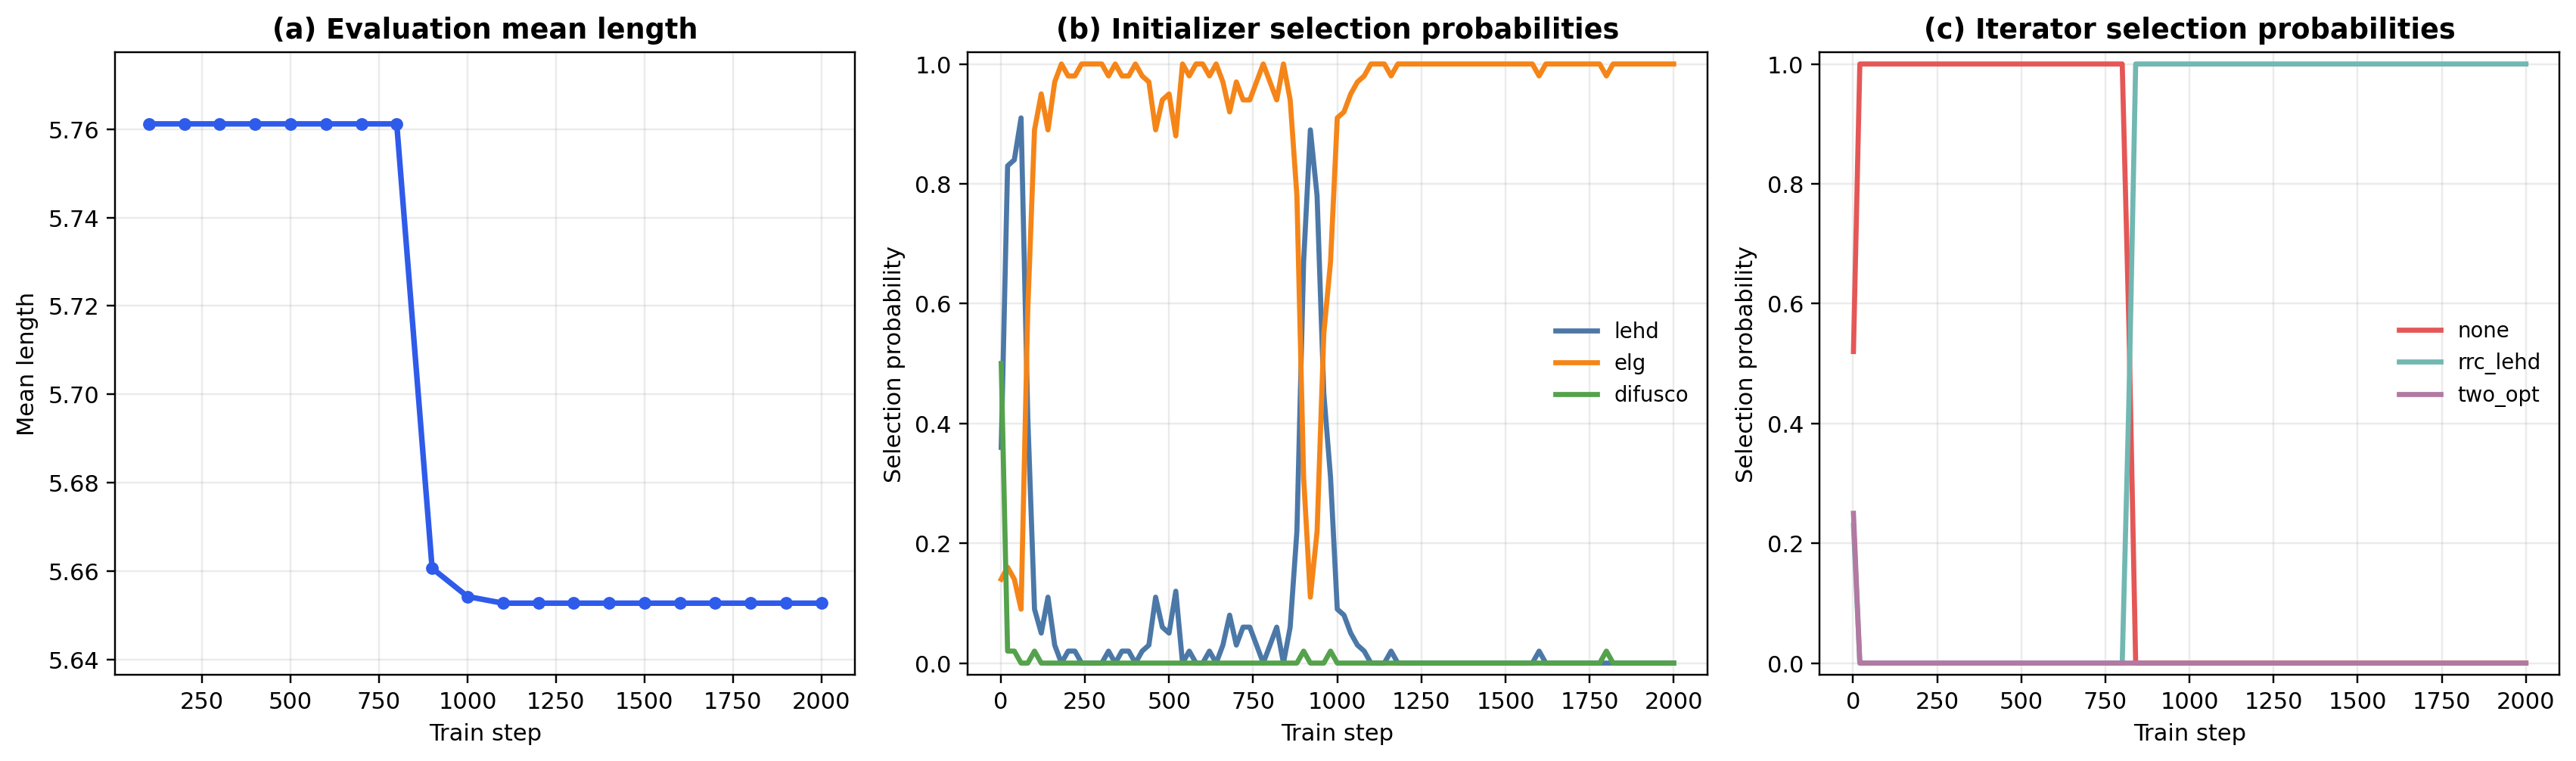
\includegraphics[width=\textwidth]{figures/research/figure-05-two-gate-collapse-triptych.png}
  \caption{双门控强化学习方法中的策略坍缩过程。左图给出评测集上的 mean length 随训练步数的变化；中图给出初始化 gate 对各候选方法的选择概率；右图给出迭代 gate 对各候选方法的选择概率。可以看到，训练后期两个 gate 都收缩到几乎确定性的单一选择，评测性能也随之进入平台期。}
  \label{fig:two-gate-collapse}
\end{figure}
